%  Typ dokumentu - článek, prezentace aj.
\documentclass[english]{article}

%  Nastaví vstupní a výstupní kódování znaků (encoding) a lokalizace
\usepackage[T1]{fontenc}
\usepackage[utf8]{inputenc}
\usepackage[english,czech]{babel}
\usepackage{icomma}

%  Formát papíru a odsazení od jeho okrajů
\usepackage[letterpaper]{geometry}
\geometry{verbose,tmargin=1.5cm,bmargin=2cm,lmargin=2cm,rmargin=2cm}

%  Umožňuje pracovat s grafikou
\usepackage{graphicx}
\usepackage{bigstrut}
\usepackage{epstopdf}

%  Automaticky odsadí i první paragraf v každé sekci
\usepackage{indentfirst}

%  Umožňuje rozdělovat obsah na více sloupců
\usepackage{multicol}
\usepackage{booktabs}
\usepackage{pgffor}
\usepackage{wrapfig}

%  Umožňuje používat hypertextové odkazy, nastavuje jejich barvu a vlastnosti
\usepackage[unicode]{hyperref}
\hypersetup{
	colorlinks=true, citecolor=blue, filecolor=blue, linkcolor=blue,
	urlcolor=blue
}

%  Umožnění odstranění italiky u jednotek
\newcommand{\unit}[1]{~\mathrm{#1}}
\newcommand{\unitb}[1]{~\mathrm{[#1]}}
\newcommand{\unitbr}[1]{\qquad\mathrm{[#1]}}


%  Formátování stránek, empty = odstraní číslování
% \pagestyle{empty}

%  Řádkování
\linespread{1.2}

%  Lepší zobrazování matematiky (rozšíření sum o \limits atd.)
%  Umožní psát přes \mathbb{N/R/Q/..} množiny čísel
\everymath{\displaystyle}
\usepackage{amsmath, amsthm, amssymb, wasysym}

%  Velikost fontu matematických výrazů v dokumentu lze pro danou
% základního fontu dokumentu upravit pomocí:
% \DeclareMathSizes{X}{Y}{Z}{U} kde:
% X je velikost fontu v dokumentu, pro kterou se matematika upraví
% Y je standartní velikost fontu matematiky
% Z je velikost fontu zmenšených (vnořených výrazů)
% U je velikost fontu ještě více zmenšených (vnořených výrazů).
\DeclareMathSizes{10}{10.5}{9}{9}

%  Nastaví autora, název, datum, skupinu měření apod. 
%  (můj vlastní příkaz, umožní znovu-použití v dokumentu)
\newcommand{\Author}{David Roesel}
\newcommand{\Coauthor}{Schönfeldová, Vyšín}
\newcommand{\Institute}{FJFI ČVUT v Praze}
\newcommand{\Subject}{VAKUOVÁ FYZIKA A TECHNIKA}
\newcommand{\Group}{Pá 14:30}
\newcommand{\Kruh}{FE}
\newcommand{\Title}{Úloha \#2  \\Čerpání difusní olejovou vývěvou}
\newcommand{\Date}{14.11.2014}

% Custom comands
\newcommand{\dd}{\mathrm{d}}
\newcommand{\dln}{\mathrm{ln}}
\newcommand{\ee}{\mathrm{e}}
\newcommand{\jelina}{Oooo, Jelina!}

% Začátek dokumentu - Formátování na výstup
\begin{document}

% Interní proměnné, možno zobrazovat u prezentací, používají se při
% generování pomocí \titlepage apod.
\author{\Author}
\title{\Title}
\date{\Date}

%  Lokalizace některých názvů do češtiny
\renewcommand{\figurename}{Obr.}
\renewcommand{\tablename}{Tab.}
\renewcommand{\refname}{Reference}

% --- Hlavička dokumentu -----------------------------------------------

\setlength{\parindent}{0cm}
\begin{multicols}{2}
\textbf{\Subject \\
        \Institute \\[0.1cm]
%\large  \Title \\[0.5cm]
\Title \\[0.5cm]
}
\begin{tabular}{rlrl}
\large Datum měření: & \Date & \large Skupina: & \Group \\
\large Jméno: & \Author & \large Kroužek:  & \Kruh\\
\large Spolupracovali: & \Coauthor &\large Klasifikace:\\
\end{tabular}

\begin{flushright}

\includegraphics[scale=0.28]{../../_meta/fjfi_standart.pdf}
\hspace{0.2cm}
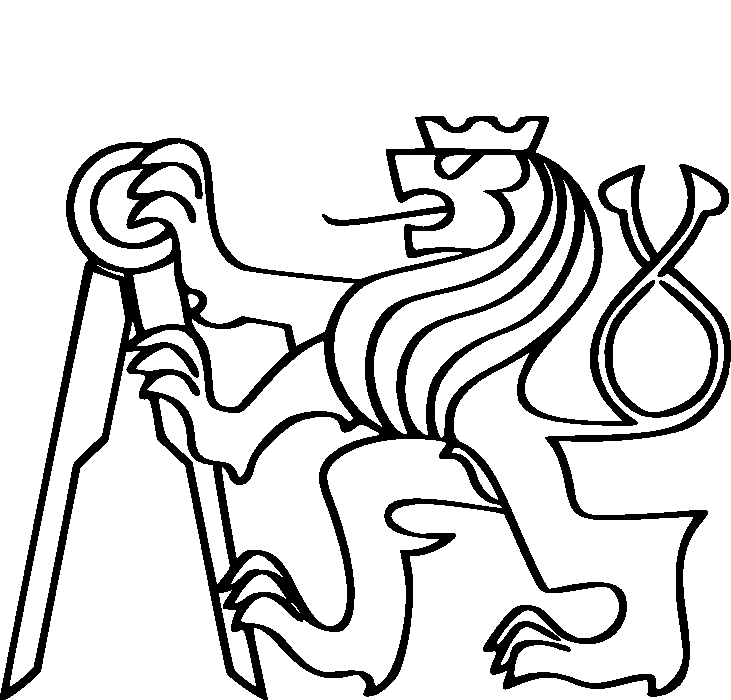
\includegraphics[scale=0.28]{../../_meta/cvut_standart.pdf}
\end{flushright}
\end{multicols}
\hrule
\vspace{0.5cm}

% ----------------------------------------------------------------------


% --- Tělo dokumentu ---------------------------------------------------
\setlength{\parindent}{0.5cm}

\section{Pracovní úkoly}
\begin{enumerate}
	\item Sledujte čerpání uzavřeného objemu difuzní olejovou vývěvou (DOV) od atmosférického až po dosažení přibližně ustáleného tlaku ($\geq$ 1 hod.).
    \item Změřte pro několik hodnot tlaku tlakový spád na cloně ($\diameter = 5\unit{mm}$, $l = 1\unit{mm}$).
	\item Ocejchujte výbojový manometr (Penning) podle ionizačního triodového vakuometru - dle situace lze zaměnit s druhým bodem (po delším čerpání  $\approx 1\unit{hod}$. pro odplynění).
	\item Z tlakového spádu na cloně určete efektivní čerpací rychlost DOV nad ventilem.
	\item Určete maximální výstupní tlak DOV. (Tlak, při němž se hroutí čerpací proces.)
\end{enumerate}

\section{Úvod}
\begin{wrapfigure}{r}{0.5\textwidth}
			\centering
			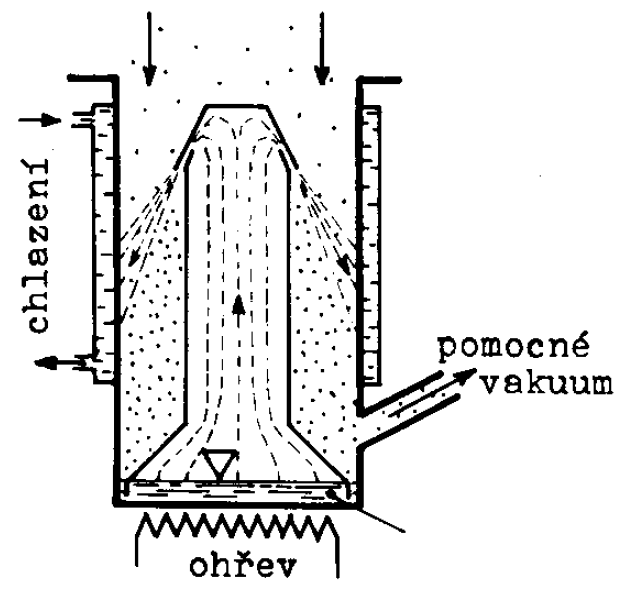
\includegraphics[width=5cm]{../att/difu_schema.png}
			\caption{Schéma difusní vývěvy (převzato z \cite{bib:praskripta}).}
			\label{fig:schema_dif}
\end{wrapfigure}
Difusní olejová vývěva (viz Obr.~\ref{fig:schema_dif}) je velmi často užívanou součástkou, která pracuje spolehlivě a dosahuje velice nízkých tlaků (mezní tlaky se typicky pohybují okolo $10^{-2}$ až $10^{-7}$ Pa). Mezi její hlavní nevýhody patří přítomnost oleje, který může lehce znečišťovat vakuum svými parami, a relativně dlouhý rozjezd, kvůli němuž je třeba čerpat delší dobu. 

Typicky je tento druh vývěv schopen pracovat od desítek Pascalů výstupního tlaku, takže je třeba jim předřadit jinou vývěvu, která z atmosferického zmenší tlak na adekvátní hodnotu. Difusní vývěva se skládá z varné části, kde se elektrickým proudem zahřívá již zmíněný olej, a z pracovní části. Vývěva musí být za provozu také chlazena (typicky vodou). 

\section{Vypracování}
  \subsection{Teoretický úvod}
  	Střední volnou dráhu molekuly ve vzduchu můžeme určit ze vztahu
	\begin{equation}
		l_{s}=6,6\cdot10^{-3}\cdot\frac{1}{p}\unitbr{m;Pa}.
	\label{eq:ls}
	\end{equation}
  	Pro vodivost tenkého otvoru o obsahu $A$ v tenké stěně při molekulárním proudění vzduchu o teplotě $20\unit{^\circ C}$ platí
  	\begin{equation}
  		C = 11,6\cdot A\unitbr{l/s;cm^2}.
  	\label{eq:Cm}
  	\end{equation}
  	
  	Uvažujme dva objemy spojené malým otvorem a v každém z nich \textit{udržovaný} určitý tlak. Předpokládejme, že se tlaky v těchto objemech nebudou rovnat. Dále platí, že plyn bude mít tendenci proudit z objemu o vyšším tlaku do objemu s tlakem nižším. Po dostatečně dlouhém čase se systém ustálí ve stavu rovnováhy. V tomto stavu bude otvorem protékat konstantní proud plynu o velikosti
  	\begin{equation}
  		q=C\cdot\Delta p,
	\label{eq:q=Cdeltap}
  	\end{equation}
  	kde $C$ je vodivost otvoru a $\Delta p=p_0-p$ je tlakový rozdíl, přičemž $p_0$, $p$ jsou vyšší a nižší tlak z obou oblastí. Pokud bude $S$ objem plynu odčerpaný vývěvou při daném tlaku za čas $t_0=1\unit{s}$, pak $p\cdot S$ bude představovat čerpané množství plynu. Předpokládáme-li dokonalé utěsnění, můžeme psát
  	\begin{equation}
  		pS=p\cdot\dfrac{\dd V}{\dd t}=-V\cdot\dfrac{\dd p}{\dd t}.
  	\label{eq:pSutesneni}
  	\end{equation}
  	Upustíme-li však od posledního předpokladu a vezmeme-li v potaz zdroje plynu v aparatuře o hodnotě proudu $q$, bude platit podoba
  	\begin{equation}
  		pS-q=-V\cdot\dfrac{\dd p}{\dd t}.
  	\label{eq:pS}
  	\end{equation}
  	Pokud se nám podaří udržet tlaky stálé, bude člen s $\frac{\dd p}{\dd t}$ nulový a po jednoduchém dosazení rovnic (\ref{eq:q=Cdeltap}) a (\ref{eq:pS}) získáme pro čerpací rychlost $S$
  	\begin{equation}
  		S=\dfrac{q}{p}=C\cdot \dfrac{\Delta p}{p}.
  	\label{eq:S}
  	\end{equation}
  	Pro efektivní čerpací rychlost $S_{EF}$ potom platí vztah
  	\begin{equation}
  		S_{EF}=\dfrac{C\cdot S}{C+S}.
  	\label{eq:Seff}
  	\end{equation}
  	V některých úkolech budeme odečítat tlak v jednotkách Torr, které můžeme na SI jednotku Pa převést pomocí následujícího vzorce \cite{bib:torr}:
  	\begin{equation}
  		1\unit{Torr} \doteq 133,32\unit{Pa}.
  	\label{eq:torr}
  	\end{equation}
  	
			
\subsection{Postup měření}
	\subsubsection{Čerpání uzavřeného objemu difusní vývěvou}
		Když jsme přišli k aparatuře, rotační olejová vývěva už běžela a aparatura byla zapojena dle schématu na Obr.~\ref{fig:schema}. Zkontrolovali jsme, že jsou všechny ventily až na V2 uzavřené a aparaturu jsme pomocí ventilu V3 zavzdušnili. Následně jsme otevřeli ventily V1 a V3 tak, aby čerpaný objem začala ROV čerpat přes vypnutou DOV (spodem). V momentu zapnutí ROV jsme začali měřit čas a sledovali jsme Piraniho vakuometr, který měřil tlak v recipientu. 
		
			\begin{figure}[h!]
			\centering
					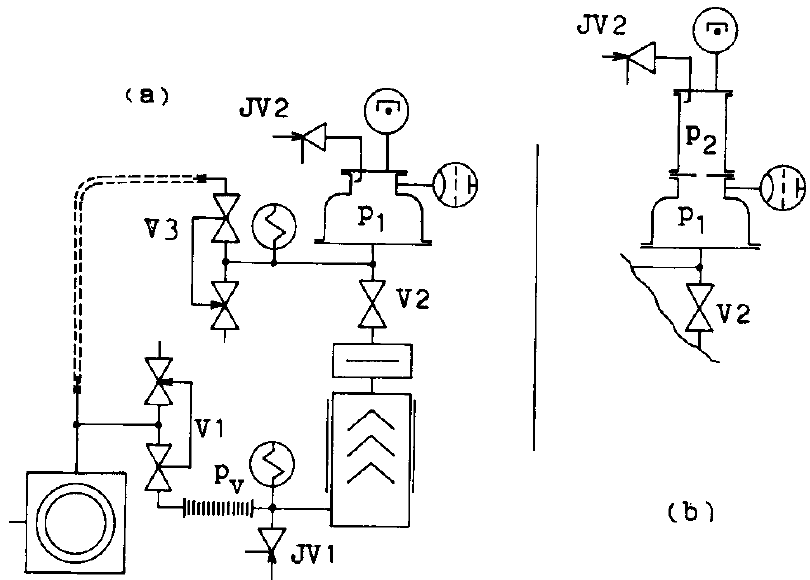
\includegraphics[width=13cm]{../att/schemata.png}
					\caption{Schéma aparatury pro měření s difusní vývěvou: (a) pro sledování čerpacího procesu DOV a měření nejvyššího výstupního tlaku, (b) úprava pro stanovení efektivní čerpací rychlosti (převzato z \cite{bib:praskripta}).}
					\label{fig:schema}
			\end{figure}
		
		Vyčkali jsme, než se tlak ustálil (na přibližném minimu, kterého zvládla dosáhnout ROV) a zapnuli jsme difusní vývěvu a chlazení. Počkali jsme, než se zahřála, a dále jsme sledovali vývoj tlaku - z počátku ještě na Piraniho vakuometru a od tlaku $10^{-2}\unit{Pa}$ na přesnějším ionizačním vakuometru. Časový průběh jsme měřili až do ustálení tlaku přibližně na hodnotě $10^{-3}\unit{Pa}$.
		
	\subsubsection{Měření tlakového spádu na clonce}
		V aparatuře byla od středeční skupiny clonka již vložena a stačilo nám jen zapnout Penningův výbojový vakuometr, který byl do aparatury zapojen nad clonku a porovnávat hodnoty na něm s těmi, které ukazoval ionizační vakuometr, který byl zapojen pod ní. Cejchování Penningova vakuometru se provádí bez clonky, takže jsme zaznamenávali údaje s vírou, že se nám ho podaří později ocejchovat a těmto údajům přiřadit korektní hodnoty. 
		
		Přes jehlový ventil JV2 jsme pomalu připouštěli do aparatury vzduch a sledovali, jak se na Penningově vakuometru hýbe ručička. V momentu, kdy se na něm ustálila hodnota, která se dala odečíst, jsme si ji zapsali spolu s hodnotou, kterou ukazoval vakuometr ionizační. Tento postup jsme opakovali pro každou možnou hodnotu na Penningově vakuometru od minimálního tlaku až po kraj stupnice.
		
		Rozměry clonky jsme později (po jejím vyndání z aparatury) změřili posuvným měřítkem.
	
	\subsubsection{Cejchování Penningova vakuometru}
		Nejprve jsme uzavřeli ventil V2 (mezi čerpaným objemem a DOV), tak aby nedošlo ke zavzdušnění DOV a pak jsme ROV pomocí ventilu V1 přepojili tak, aby čerpala objem. Stejně jako v prvním úkolu jsme přes V3 zavzdušnili vrchní část aparatury a opatrně jsme vyměnili clonku za těsnicí kroužek, který jsme nejprve očistili isopropylalkoholem. Při šroubování jsme si dávali pozor, abychom všechny šrouby utahovali postupně a nezkroutili tak gumové těsnění.  
		
		Poté jsme přes ventil V3 nechali odčerpat recipient ROV a po dostatečném poklesu tlaku jsme pomocí ventilu V1 nechali ROV opět čerpat DOV, které jsme otevřeli přístup do recipientu pomocí V2. Poté jsme nechali DOV vyčerpat objem do stejných tlaků jako při minulém úkolu a stejně jako při měření tlakového spádu jsme za otevírání JV2 pro co nejvíce hodnot zjišťovali, jaký tlak na ionizačním vakuometru odpovídá ryskám na vakuometru Penningově. 
	
	\subsubsection{Měření maximálního výstupního tlaku DOV}
		V této části jsme hledali maximální výstupní tlak, při kterém čerpací proces DOV ještě funguje. Výstupní tlak jsme zvyšovali otevíráním ventilu JV1 a čekali jsme, kdy zakolísá ručička na Penningově vakuometru. V ten moment jsme odečetli hodnotu z Piraniho vakuometru, uzavřeli JV1, počkali na ustálení tlaku a měření opakovali.

\subsection{Naměřené hodnoty}

	\subsubsection{Čerpání uzavřeného objemu difusní vývěvou}
		Naměřené hodnoty pro čerpání uzavřeného objemu difusní vývěvou jsou zaneseny do Tab.~\ref{tab:tlak} a vyneseny do grafu na Obr.~\ref{fig:g_tlak}. Minimální tlak, jakého jsme pomocí DOV byli schopni dosáhnout, byl 
		\begin{equation}
			p_{min} = 1,6\cdot10^{-3}\unit{Pa}.
		\label{eq:pmin}
		\end{equation}
	
	\subsubsection{Tlakový spád na clonce}
		Změřené rozměry clonky (průměr otvoru $\diameter$ a tloušťku clonky $h$) jsme posuvným měřítkem určili jako 
		\begin{equation}
			\begin{aligned}
				\diameter &= (4,9\pm0,1)\unit{mm},\\
				        h &= (1,0\pm0,1)\unit{mm},
			\end{aligned}
		\end{equation}
		kde jako chybu bereme nejmenší dílek měřítka.
		
		Obsah clonky $S_c$ poté určíme jednoduše jako obsah kruhu $S=\pi (\diameter/2)^2$ s chybou podle (\ref{eq:chyba_neprime_mereni}) na
		\begin{equation}
			S_c = (18,9 \pm 0,8)\unit{mm^2}.
		\end{equation}
		
		Vodivost $C$ pak lze spočítat za předpokladu tenké clonky a odpovídající teploty pomocí (\ref{eq:Cm}) jako
		\begin{equation}
			C \approx 2,2\unit{l\cdot s^{-1}}.
		\end{equation}
		
		Naměřené a vypočítané hodnoty pro měření tlakového spádu na clonce jsou zaneseny do Tab.~\ref{tab:clonka}. Čerpací rychlost $S$ jsme spočítali pomocí (\ref{eq:S}) a  efektivní čerpací rychlost $S_{EF}$ pak podle (\ref{eq:Seff}).
	
	\subsubsection{Cejchování Penningova vakuometru}
		Naměřené hodnoty jsou zaneseny v Tab.~\ref{tab:cejchovani}. Cejchování jsme provedli pouze pro ty hodnoty, které ještě byly změřitelné na rozsahu ionizačního vakuometru. 

	\subsubsection{Měření maximálního výstupního tlaku DOV}
		Naměřené hodnoty jsou zaneseny do Tab.~\ref{tab:max}. Průměrný tlak, při kterém se zhroutí čerpací proces DOV, jsme určili pomocí (\ref{eq:aritmeticky_prumer}) s chybou podle (\ref{eq:chyba_aritmetickeho_prumeru}) jako
		\begin{equation}
			p_{hr} = (18,8\pm0,4)\unit{Pa}.
			\label{eq:phr}
		\end{equation}
			
	\subsection{Diskuse}
		
		\subsubsection{Čerpání uzavřeného objemu difusní vývěvou}
			Čerpání pomocí ROV probíhalo stejně jako při měření v předchozí úloze. Bylo vidět (viz Obr.~\ref{fig:g_tlak}), že kolem dvanácté minuty se tlak začal ustalovat a jen pomocí ROV už by se ho nepodařilo příliš snížit. Na grafu je jasně patrný nástup čerpání difusní olejovou vývěvou, která následně znovu tlak řádově snížila.
			
			Prvním z pozorovaných jevů je, že se tlak začal snižovat až určitý čas po zapnutí DOV (řádově minuty), což se dá přisoudit postupnému zahřívání vývěvy, respektive oleje v ní. Po chvíli (ještě než se zahřála úplně) přestal tlak být konstantní, ale lehce kolísal. To přisuzujeme tomu, že se z oleje při zahřívání uvolňovaly plyny, které se na něj navázaly. Jakmile se olej dostatečně ohřál a plyny se z něj uvolnily, začala DOV prudce snižovat tlak až na řádově $10^{-2}$ Pa, kde se pokles tlaku opět zpomalil, takže napodobil křivku čerpání ROV.
			
			V grafu na Obr.~\ref{fig:g_tlak} by se mohlo zdát, že pomyslná křivka postupně klesá až na nejnižší tlak a že osamocený bod na grafu je chybou měření. S jistotou můžeme říci, že tomu tak není, jelikož jsme měrky sledovali po celou dobu a zaznamenávali pouze rysky na Piraniho manometru, u kterých víme přesnou hodnotu. Kdybychom měli jiný přístroj na měření tlaků v tomto rozsahu, mohli bychom do grafu zanést větší množství bodů.
			
			Průběh by se dal naměřit pro ještě nižší tlaky, pokud bychom se rozhodli čekat déle. Vzhledem k době, jakou nám trvalo vyčerpat aparaturu na tento tlak, a k tomu, že jsme potřebovali provést i jiná měření, jsme se rozhodli nečekat na úplné odplynění aparatury. Minimální tlak, kterého jsme dosáhli, tedy nemůžeme nazývat mezním.
		
		\subsubsection{Tlakový spád na clonce}
			Stejně jako při úloze s ROV bylo i při tomto měření obtížné jehlovým ventilem přesně nastavit tlak na Penningově vakuometru. Nakonec jsme byli nuceni opět pouze nechat ručičku konat velice pomalý pohyb a odečíst tlak v momentu, kdy přecházela rysku, kterou jsme chtěli měřit. 
			
			Nutno je také poznamenat, že na konci tohoto měření došlo ke spálení katody v ionizačním vakuometru, který přímo ovlivňuje všechny výpočty v tomto úkolu. Cejchování Penningova vakuometru, který je taktéž využíván pro každý z výpočtů, bylo tím pádem prováděno s jinou katodou a nebylo tedy vykonáváno za stejných podmínek. Nemůžeme si tak být zcela jisti, že jsme opravdu ocejchovali ty samé hodnoty jako při tomto měření.
			
			Z některých tlaků naměřených se clonkou jsme nemohli určit $S_{EF}$ vzhledem k tomu, že pro tyto hodnoty nešel ocejchovat Penningův vakuometr. To bylo způsobeno tím, že se dané tlaky pohybovaly mimo rozsah ionizačního vakuometru. Z výsledků můžeme říci, že je $S_{EF}$ za klesajícího tlaku buď konstantní, nebo lehce klesá. V prvním případě by to znamenalo, že jsme se ještě nepřiblížili dostatečně k meznímu tlaku. Ve druhém pak, že se meznímu tlaku blížíme a námi naměřené hodnoty odpovídají teorii.
	
		\subsubsection{Měření maximálního výstupního tlaku DOV}
			Při měření maximálního výstupního tlaku DOV bylo jasně vidět, jak nepřesný je Piraniho vakuometr. Hodnoty maximálního tlaku, který jsme mohli pomocí ventilu nastavit, jsme odhadovali pouze na několika milimetrech mezi měrkou 10 a 20 Pa a měli jsme z ní určovat hodnoty kolem 18 - tedy zcela nepřesně. Pokud bychom korektně zohlednili tuto situaci, mohli bychom říct, že je $p_{hr} = 15-20\unit{Pa}$. Řekneme-li, že jsme schopni určit hodnotu s přesností na 0,5 Pa, bude platit již zmíněný výsledek (\ref{eq:phr}).
			
		\emph{Pozn.: Ukázalo se, že se clonka nedá brát jako tenká, takže výpočty zde nejsou dobře. Takžtéž $S_{EF}$ by se mělo značit $S_{EFt}$ a $S$ zase $S_{EF}$.}
						
\section{Závěr}
	Sledovali jsme 70 minut čerpání uzavřeného objemu difusní olejovou vývěvou (DOV) od atmosferického až po dosažení přibližně ustáleného tlaku $p_{min}=1,6\cdot 10^{-3}\unit{Pa}$. 
	
	Pro několik hodnot tlaku jsme změřili tlakový spád na cloně.
	
	Ocejchovali jsme výbojový manometr (Penning) podle ionizačního triodového vakuometru.
	
	Z tlakového spádu na cloně jsme určili efektivní čerpací rychlost DOV nad ventilem jako řádově litry za sekundu.
	
	Určili jsme maximální výstupní tlak DOV (tlak, při kterém se hroutí čerpací proces) jako $p_{hr} = (18,8\pm0,4)\unit{Pa}$.
	
\section {Použitá literatura}
% --- Literatura a reference -------------------------------------------
\begingroup
\renewcommand{\section}[2]{}

\begin{thebibliography}{9}

\bibitem{bib:chyby} Kolektiv KF, \emph{Chyby měření} [Online], [cit. \today] \newline http://praktikum.fjfi.cvut.cz/documents/chybynav/chyby-o.pdf

\bibitem{bib:praskripta}Král, J.: \emph{Cvičení z vakuové techniky},
Vydavatelství ČVUT, Praha, 1996

%\bibitem{bib:tlak}ČHMÚ: \emph{Aktuální informace o počasí na území České republiky}, {[}online{]}, {[}cit. \today{]},\newline http://pr-asv.chmi.cz/synopy-map/pocasisp.php?ukazatel=stanice\&pozadi=\&pozadi=mapareg\&graf=ano
 
\bibitem{bib:torr}Thompson, A.: \emph{Guide for the Use of the International System of Units (SI)} [Online], [cit \today] \newline
http://physics.nist.gov/cuu/pdf/sp811.pdf
 

\end{thebibliography}
\endgroup
% ----------------------------------------------------------------------
\setcounter{equation}{0}
\numberwithin{equation}{section}

\clearpage
\part*{Přílohy}

%\section{Domácí příprava}
%	Domácí příprava je přiložena k protokolu.
%\clearpage
\section{Statistické zpracování dat}
	Pro statistické zpracování využíváme aritmetického průměru:
	\begin{equation} \label{eq:aritmeticky_prumer}
	\overline{x} = \frac{1}{n}\sum\limits_{i=1}^{n}x_i,
	\end{equation}

%	jehož směrodatnou odchylku spočítáme jako 
%	\begin{equation} \label{eq:smodch_aritmetickeho_prumeru}
%	\sigma_0 = \sqrt{\frac{1}{n} \sum\limits_{i=1}^{n}\left( x_i - \overline{x} \right)^2 },
%	\end{equation}
%	
%	kde $ x_i $ jsou jednotlivé naměřené hodnoty, $ n $ je počet měření, $ \overline{x} $ aritmetický průměr a $ \sigma_0 $ jeho chyba \cite{bib:chyby}.
	
	
	jehož chybu spočítáme jako 
	\begin{equation} \label{eq:chyba_aritmetickeho_prumeru}
	\sigma_0 = \sqrt{\frac{1}{n(n-1)} \sum\limits_{i=1}^{n}\left( x_i - \overline{x} \right)^2 },
	\end{equation}
	
	kde $ x_i $ jsou jednotlivé naměřené hodnoty, $ n $ je počet měření, $ \overline{x} $ aritmetický průměr a $ \sigma_0 $ jeho chyba \cite{bib:chyby}.
%	
Při nepřímém měření počítáme hodnotu s chybou dle následujících vztahů:
	\begin{equation}
	u = f(x, y, z, \ldots),
	\end{equation}
	\begin{displaymath}
	x = (\overline{x} \pm \sigma_x), \qquad
	y = (\overline{y} \pm \sigma_y), \qquad
	z = (\overline{z} \pm \sigma_z), \qquad
	\ldots,
	\end{displaymath}
	
	kde $ u $ je veličina, kterou určujeme nepřímo z měřených veličin $ x, y, z, \ldots $ 
	
	Pak
	\begin{displaymath}
	\overline{u} = f(\overline{x}, \overline{y}, \overline{z}, \ldots),
	\end{displaymath}
	\begin{equation}\label{eq:chyba_neprime_mereni}
	\sigma_u = \sqrt{\left( \frac{\partial f}{\partial x} \right)^2 \sigma^2_x + \left( \frac{\partial f}{\partial y} \right)^2 \sigma^2_y + \left( \frac{\partial f}{\partial z} \right)^2 \sigma^2_z + \ldots},
	\end{equation}
	\begin{displaymath}
	u = (\overline{u} \pm \sigma_ u).
	\end{displaymath}
%%	
%V případě, že máme několik různě přesných měření stejné veličiny, používáme vztah pro vážený průměr:
%	\begin{equation} 
%	\overline{x}=\frac{\sum\limits_{i=1}^{n}p_{i}x_{i}}{\sum\limits_{i=1}^{n}p_{i}},
%	\end{equation}
%	
%	kde $\overline{x}$ je vážený průměr, $x_{i}$ jsou jednotlivá měření a pro $p_{i}$ platí
%	 
%	\begin{equation}
%	p_{i}=\frac{1}{\sigma_{i}^{2}},
%	\end{equation}
%	
%	kde $\sigma_{i}$ jsou jednotlivé chyby daných měření.
%	 
%	Celkovou chybu tedy vypočítáme ze vztahu
%	\begin{equation} \label{eq:vazeny_prumer}
%	\sigma_{0}=\sqrt{\frac{1}{\sum\limits_{i=1}^{n}p_{i}}}.
%	\end{equation}
%
%\subsubsection{Metoda nejmenších čtverců}
%Snažíme-li se metodou nejmenších čtverců proložit data lineární závislostí $Y_i = ax_i+b$, dosazujeme hodnoty $x_i, y_i$ a snažíme se najít parametry $a$ a $b$ tak, aby byl součet všech kvadratických odchylek $\Delta Y_i^2$ minimální. Toho dosáhneme pomocí následujících vzorců \cite{bib:ctverce} :
%\begin{equation}\label{eq:ctverce_a}
%		a = \frac{n\sum\limits_{i=1}^{n}{x_i y_i}  - \sum\limits_{i=1}^{n}{x_i}\sum\limits_{i=1}^{n}{y_i}}{n\sum\limits_{i=1}^{n}{x_i^2}  - \left(\sum\limits_{i=1}^{n}{x_i}\right)^2}, \qquad \qquad
%		\sigma_a = \sqrt{\frac{n\sum\limits_{i=1}^{n}{(y_i - Y_i)^2} }{(n-2)\left(\sum\limits_{i=1}^{n}{x_i^2}  - \left(\sum\limits_{i=1}^{n}{x_i}\right)^2\right)}},
%\end{equation}
%
%\begin{equation}\label{eq:ctverce_b}
%		b = \frac{\sum\limits_{i=1}^{n}{x_i^2} \sum\limits_{i=1}^{n}{y_i}  - \sum\limits_{i=1}^{n}{x_i}\sum\limits_{i=1}^{n}{x_i y_i}}{n\sum\limits_{i=1}^{n}{x_i^2}  - \left(\sum\limits_{i=1}^{n}{x_i}\right)^2}, \qquad \qquad
%		\sigma_b = \sqrt{\frac{\sum\limits_{i=1}^{n}{x_i^2}\sum\limits_{i=1}^{n}{(y_i - Y_i)^2} }{n(n-2)\left(\sum\limits_{i=1}^{n}{x_i^2}  - \left(\sum\limits_{i=1}^{n}{x_i}\right)^2\right)}}.
%\end{equation}
	
\clearpage

\subsection{Tabulky a grafy}

\begin{table}[htbp]
\catcode`\-=12 % HAX na enable cline v českym bable
  \centering
    \begin{tabular}{|r|r|r|r|}
    \hline
    \boldmath{}\textbf{$t\unit{[s]}$}\unboldmath{} & \boldmath{}\textbf{$p_p\unit{[Pa]}$}\unboldmath{} & \boldmath{}\textbf{$t\unit{[s]}$}\unboldmath{} & \boldmath{}\textbf{$p_i\unit{[Pa]}$}\unboldmath{} \bigstrut\\
    \hline
    0,00  & 5,00E+04 & 1035,00 & 1,13E-02 \bigstrut\\
    \hline
    6,01  & 2,00E+04 & 1146,24 & 7,33E-03 \bigstrut\\
    \hline
    14,32 & 1,00E+04 & 1190,22 & 6,67E-03 \bigstrut\\
    \hline
    22,50 & 5,00E+03 & 1318,71 & 5,33E-03 \bigstrut\\
    \hline
    32,15 & 2,00E+03 & 1581,62 & 4,00E-03 \bigstrut\\
    \hline
    39,45 & 1,00E+03 & 2118,29 & 3,33E-03 \bigstrut\\
    \hline
    46,23 & 5,00E+02 & 3001,71 & 2,00E-03 \bigstrut\\
    \hline
    53,36 & 2,00E+02 & 4151,99 & 1,60E-03 \bigstrut\\
    \hline
    62,37 & 1,00E+02 & \multicolumn{1}{r}{} & \multicolumn{1}{r}{} \bigstrut\\
\cline{1-2}    69,12 & 5,00E+01 & \multicolumn{1}{r}{} & \multicolumn{1}{r}{} \bigstrut\\
\cline{1-2}    86,60 & 2,00E+01 & \multicolumn{1}{r}{} & \multicolumn{1}{r}{} \bigstrut\\
\cline{1-2}    139,57 & 1,00E+01 & \multicolumn{1}{r}{} & \multicolumn{1}{r}{} \bigstrut\\
\cline{1-2}    764,35 & 5,00E+00 & \multicolumn{1}{r}{} & \multicolumn{1}{r}{} \bigstrut\\
\cline{1-2}    \end{tabular}%
  
  \caption{Naměřené hodnoty tlaku v závislosti na čase $t$. Tlaky $p_p$ byly naměřeny Piraniho vakuometrem při čerpání pomocí ROV, tlaky $p_i$ potom ionizačním vakuometrem po zapnutí DOV a byly převedeny na Pa pomocí (\ref{eq:torr}).}
  
  \label{tab:tlak}%
\end{table}%


\begin{figure}[h!]
	\begin{center}
		\vspace*{-0.5cm}
		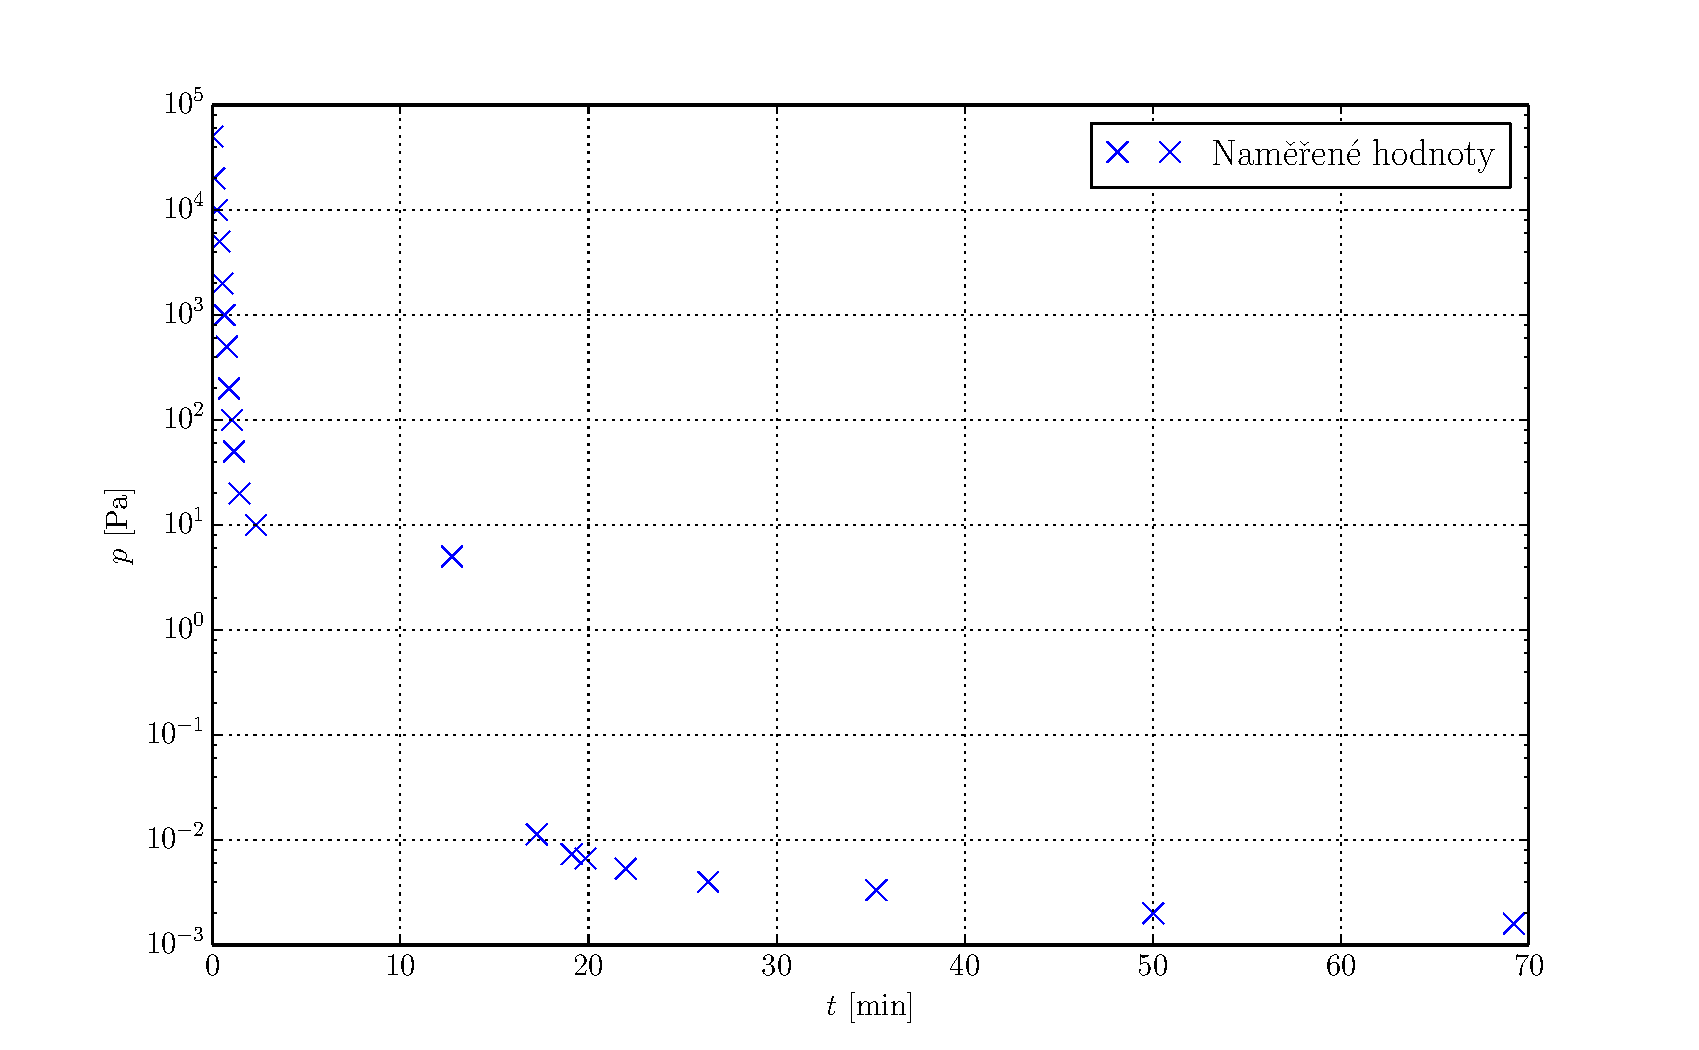
\includegraphics[width=\linewidth]{../plt/01_p.pdf}
		\vspace*{-0,7cm}
		\caption{Graf závislosti tlaku v recipientu $p$ na čase $t$. Difusní vývěvu jsme zapnuli zhruba ve 13. minutě. Osamocená hodnota kolem 11. minuty není chyba měření, viz diskuse.}
		\label{fig:g_tlak}
	\end{center}
\end{figure}

\begin{table}[htbp]
\catcode`\-=12 % HAX na enable cline v českym bable
  \centering
      
          \begin{tabular}{|r|r|r|r|r|r|r|}
          \hline
          \boldmath{}\textbf{$p_p\unitb{-}$}\unboldmath{} & \boldmath{}\textbf{$p_i\unitb{Torr}$}\unboldmath{} & \boldmath{}\textbf{$p_p\unitb{Pa}$}\unboldmath{} & \boldmath{}\textbf{$p_i\unitb{Pa}$}\unboldmath{} & \boldmath{}\textbf{$\Delta p\unitb{Pa}$}\unboldmath{} & \boldmath{}\textbf{$S\unitb{l/s}$}\unboldmath{} & \boldmath{}\textbf{$S_{EF}\unitb{l/s}$}\unboldmath{} \bigstrut\\
          \hline
          1,00E-02 & 1,20E-05 & 0,009 & 0,002 & 0,007 & 9,5   & 1,8 \bigstrut\\
          \hline
          2,00E-02 & 1,60E-05 & 0,017 & 0,002 & 0,015 & 14,9  & 1,9 \bigstrut\\
          \hline
          5,00E-02 & 2,60E-05 & 0,029 & 0,003 & 0,026 & 16,3  & 1,9 \bigstrut\\
          \hline
          1,00E-01 & 4,50E-05 & \multicolumn{1}{r}{} & \multicolumn{1}{r}{} & \multicolumn{1}{r}{} & \multicolumn{1}{r}{} & \multicolumn{1}{r}{} \bigstrut\\
      \cline{1-2}    2,00E-01 & 9,00E-05 & \multicolumn{1}{r}{} & \multicolumn{1}{r}{} & \multicolumn{1}{r}{} & \multicolumn{1}{r}{} & \multicolumn{1}{r}{} \bigstrut\\
      \cline{1-2}    5,00E-01 & 2,00E-04 & \multicolumn{1}{r}{} & \multicolumn{1}{r}{} & \multicolumn{1}{r}{} & \multicolumn{1}{r}{} & \multicolumn{1}{r}{} \bigstrut\\
      \cline{1-2}    \end{tabular}%  
  
    \caption{Naměřené a vypočítané hodnoty při měření tlakového spádu na clonce. $p_p$ je tlak nad clonkou (měřený Penningovým vakuometrem), $p_i$ tlak pod ní (měřený ionizačním vakuometrem). Oba tlaky $p_p$ i $p_i$ byly převedeny do jednotek Pa pomocí hodnot z Tab.~\ref{tab:cejchovani} a (\ref{eq:torr}). $\Delta p$ je dále jejich rozdíl, $S$ čerpací rychlost vypočítaná pomocí (\ref{eq:S}) a $S_{EF}$ efektivní čerpací rychlost vypočítaná pomocí (\ref{eq:Seff}). Chyby měření byly zanedbány vzhledem k nepřesnosti vztahů a naměřených hodnot.}
    \label{tab:clonka}%
\end{table}%


\begin{table}[htbp]
  \centering
    \begin{tabular}{|r|r|r|}
    \hline
    \boldmath{}\textbf{$p\unit{[Torr]}$}\unboldmath{} & \boldmath{}\textbf{$p\unit{[Pa]}$}\unboldmath{} & \boldmath{}\textbf{$p_p\unit{[-]}$}\unboldmath{} \bigstrut\\
    \hline
    6,40E-05 & 8,53E-03 & 1,00E-02 \bigstrut\\
    \hline
    1,25E-04 & 1,67E-02 & 2,00E-02 \bigstrut\\
    \hline
    2,20E-04 & 2,93E-02 & 5,00E-02 \bigstrut\\
    \hline
    \end{tabular}%
  \caption{
  Naměřené hodnoty tlaku $p$ na ionizačním vakuometru a tlaku $p_p$ na Penningově vakuometru při cejchování druhého z nich. Hodnoty $p$ byly převedeny z jednotek Torr na Pa dle (\ref{eq:torr}).}
    \label{tab:cejchovani}%
\end{table}%

\begin{table}[htbp]
\catcode`\-=12 % HAX na enable cline v českym bable
  \centering
      \begin{tabular}{|r|r|}
  \cline{2-2}    \multicolumn{1}{r|}{} & \boldmath{}\textbf{$p_{hr}\unitb{Pa}$}\unboldmath{} \bigstrut\\
  \cline{2-2}    \multicolumn{1}{r|}{} & 20 \bigstrut\\
  \cline{2-2}    \multicolumn{1}{r|}{} & 18 \bigstrut\\
  \cline{2-2}    \multicolumn{1}{r|}{} & 19 \bigstrut\\
  \cline{2-2}    \multicolumn{1}{r|}{} & 18 \bigstrut\\
  \cline{2-2}    \multicolumn{1}{r|}{} & 19 \bigstrut\\
      \hline
      \boldmath{}\textbf{$\overline{p_{hr}}\pm\sigma_{\overline{p_{hr}}}$}\unboldmath{} & $18,8\pm0,4$ \bigstrut\\
      \hline
      \end{tabular}%
  
  \caption{Naměřené hodnoty tlaků $p_{hr}$, při kterých se hroutí čerpací proces DOV. $\overline{p_{hr}}\pm\sigma_{\overline{p_{hr}}}$ je aritmetický průměr (\ref{eq:aritmeticky_prumer}) s chybou podle (\ref{eq:chyba_aritmetickeho_prumeru}).}
  \label{tab:max}%
\end{table}%



%\clearpage
%\subsection{Schémata}
%	
%	\begin{figure}[h!]
%	\centering
%			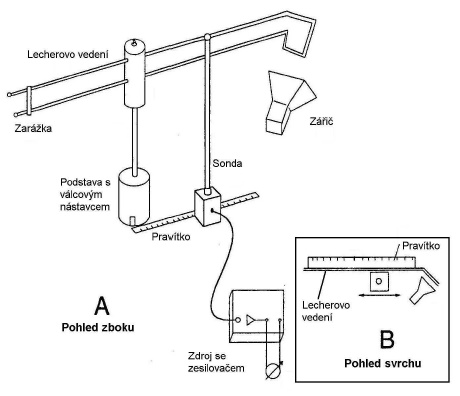
\includegraphics[width=13cm]{att/lecherovo_vedeni.jpg}
%			\caption{Experiment s Lecherovým vedením (převzato z  \cite{bib:zadani}). }
%			\label{fig:lecherovo_vlneni}
%	\end{figure}	
%	
%\clearpage
% --- Konec dokumentu --------------------------------------------------

\end{document}

